\title{Buku Tugas Akhir ITS}
\author{Musk, Elon Reeve}
% Pengaturan ukuran teks dan bentuk halaman dua sisi
\documentclass[12pt,twoside]{report}
\input{Init/Init.tex}
%========================================
%Template ini di modifikasi oleh departement Teknik Komputer ITS
%dari template yang telah dibuat Musk, Elon Reeve
%=======================================

%=======================================
%Direktori Penting 
%1. Init : Berisi File penting terkait dengan konfigurasi .
%            Isi dari direktori ini jangan diubah
%2.KataPengantar 
%3. Abstrak : berisi abstrak untuk bahasa indonesia dan bahasa inggris 
%4. Bab1-Bab5 : Isi tiap-tiap bab
%5. Pustaka : Berisi daftar pustaka 
%6. Biografi penulis 
%=======================================

%========================================
% Identutas Mahasiswa} 
%========================================
\NamaMahasiswa{Mahija Ibad Pradipta}{5024 22 1026}
\NamaMahasiswadua{Alif Ridhwan Al Ghozali}{5024 22 1034}
%========================================
%Identitas Tugas Akhir
%========================================
\KodeMataKuliah{xxx}
\JudulTAInd{Pengembangan Sistem Pemantauan Cerdas Berbasis Pengolahan Citra Digital Menggunakan ESP32-CAM dengan Pemrosesan pada Server Intel NUC}
\JudulTAEng{AUTONOMOUS HUMAN SEARCH SYSTEM USING A HOLYBRO S500 DRONE WITH A FIXED MONOCULAR CAMERA BASED ON RASPBERRY PI 5}
\Tempat{Surabaya}
%========================================
% Daftar Pembimbing 
%========================================
\PembimbingSatu{Dr. Arief Kurniawan, S.T., M.T}{19740907 200212 1 001} 
\PembimbingDua{Dr. Eko Mulyanto Yuniarno, S.T., M.T.}{19680601 199512 1 009} 
%========================================
% Daftar Penguji
%========================================
\PengujiSatu{Arta Kusuma Hernanda, S.T., M.T}{1996202311024} 
\PengujiDua{Dr. Diah Puspito Wulandari, S.T., M.Sc.}{19801219200501 2 001} 
\PengujiTiga{Bambang Widjanarko, S.T., M.T}{} 

%========================================
%Identitas Departement dan fakultas
%========================================
\KepalaDepartemen{Dr. Arief Kurniawan, S.T., M.T}{19740907200212 1 001} 
\Departemen{Teknik Komputer}{Computer Engineering}
\Fakultas{Teknologi Elektro dan Informatika Cerdas}{Intelligent Electrical And Informatics Technology}
\SingkatanFakultas{FTEIC}{FIEI}


% Isi keseluruhan dokume
\begin{document}
\input{Init/TataLetak.tex} 

% Bab 1 pendahuluan
\begin{spacing}{1.2}
	\chapter{PENDAHULUAN}
\end{spacing}

\pagenumbering{arabic}
\vspace{4ex}

\section{Latar Belakang}
Perkembangan teknologi Internet of Things (IoT) memungkinkan berbagai perangkat untuk saling terhubung dan bertukar data melalui jaringan internet. Salah satu implementasi IoT yang banyak digunakan adalah sistem monitoring berbasis kamera yang dapat digunakan untuk mendukung keamanan dan pengawasan suatu lingkungan.

ESP32-CAM merupakan salah satu perangkat yang banyak dimanfaatkan dalam pengembangan sistem monitoring karena memiliki modul kamera dan konektivitas Wi-Fi dalam satu perangkat dengan biaya yang relatif rendah. Namun, sistem monitoring berbasis kamera memerlukan infrastruktur yang mampu mengelola pengiriman data, penyimpanan gambar, pemantauan kondisi perangkat, serta penyajian informasi kepada pengguna secara real-time.

Pada penelitian ini dikembangkan sebuah platform monitoring CCTV berbasis ESP32-CAM yang terintegrasi dengan website dan aplikasi mobile. Sistem memanfaatkan protokol MQTT untuk komunikasi data antar perangkat dan WebSocket untuk menampilkan pembaruan data secara real-time pada website tanpa mekanisme polling. Data hasil tangkapan kamera disimpan pada object storage, sedangkan informasi perangkat dan aktivitas sistem disimpan pada basis data terpusat.

Selain itu, sistem dilengkapi dengan fitur motion detection untuk mendeteksi adanya aktivitas pada area pengawasan, monitoring telemetri perangkat untuk mengetahui kondisi kamera secara real-time, serta notifikasi mobile yang dapat memberikan informasi kepada pengguna ketika terjadi aktivitas yang terdeteksi oleh sistem. Seluruh layanan dijalankan pada server Intel NUC menggunakan teknologi containerisasi sehingga memudahkan proses pengelolaan dan pengembangan sistem.

\section{Rumusan Masalah}
Berdasarkan uraian latar belakang di atas, rumusan masalah dalam penelitian ini didefinisikan secara lebih spesifik sebagai berikut:
\begin{enumerate}
	\item Bagaimana merancang dan mengimplementasikan platform monitoring CCTV berbasis ESP32-CAM yang dapat diakses melalui website dan aplikasi mobile secara real-time?
	\item Bagaimana membangun mekanisme komunikasi data dan penyimpanan terpusat menggunakan MQTT, WebSocket, dan server Intel NUC sehingga sistem dapat berjalan secara stabil dan efisien?
	\item Bagaimana mengimplementasikan fitur motion detection, notifikasi mobile, dan monitoring kondisi perangkat untuk mendukung proses pengawasan dan pengelolaan sistem?
\end{enumerate}

\section{Tujuan Penelitian}
Sejalan dengan rumusan masalah, penelitian ini bertujuan untuk:
\begin{enumerate}
	\item Menghasilkan rancang bangun perangkat keras dan kelistrikan sistem drone otonom yang mampu menyuplai daya komputasi secara stabil bagi perangkat \textit{edge} Raspberry Pi 5 tanpa memicu \textit{voltage sag}.
	\item Mengevaluasi performa iterasi model YOLOv8n format ONNX yang dijalankan pada sistem operasi \textit{headless} untuk meraih keseimbangan \textit{framerate} (FPS) dan latensi terbaik.
	\item Membangun mesin logika otonom tipe \textit{Persistent Multi-Target Scouting} berbasis MAVSDK yang memampukan wahana untuk menavigasi, mendokumentasi korban, dan menghindari pelacakan target duplikat secara mandiri.
\end{enumerate}

\section{Batasan Masalah}
Agar ruang lingkup penelitian tetap terarah dan terukur, ditetapkan batasan masalah sebagai berikut:
\begin{enumerate}
	\item Sistem monitoring menggunakan perangkat ESP32-CAM yang terhubung ke server melalui jaringan internet menggunakan protokol MQTT.
	
	\item Sistem terdiri dari website monitoring real-time berbasis WebSocket dan aplikasi mobile yang digunakan untuk pemantauan serta penerimaan notifikasi.
	
	\item Penyimpanan data menggunakan MySQL untuk metadata dan MinIO Object Storage untuk penyimpanan citra hasil tangkapan kamera.
	
	\item Fitur yang dikembangkan meliputi motion detection, monitoring telemetri perangkat (RSSI, uptime, free heap, dan status perangkat), serta pengiriman notifikasi kepada pengguna.
	
	\item Infrastruktur sistem dijalankan pada server Intel NUC berbasis Debian 12 dengan dukungan Docker, Cloudflared Tunnel, dan Webmin untuk pengelolaan layanan.
\end{enumerate}

\section{Manfaat Penelitian}
Penelitian ini diharapkan dapat memberikan kontribusi dan manfaat sebagai berikut:

\begin{enumerate}
	\item Bagi pengguna dan pengelola sistem, penelitian ini menghasilkan platform monitoring CCTV berbasis IoT yang memungkinkan pemantauan kondisi kamera, penerimaan notifikasi aktivitas secara real-time, serta pengelolaan perangkat dan layanan melalui website maupun aplikasi mobile.
	
	\item Bagi pengembangan teknologi, penelitian ini dapat menjadi referensi dalam pengembangan sistem monitoring berbasis IoT yang memanfaatkan ESP32-CAM, MQTT, WebSocket, motion detection, dan infrastruktur server terpusat untuk mendukung implementasi sistem pengawasan yang lebih efektif dan mudah dikembangkan di masa mendatang.
\end{enumerate}
\cleardoublepage
\chapter{KAJIAN PUSTAKA}
\label{sec:chap2_kajian_pustaka}

\section{Hasil Penelitian Terdahulu}

Penelitian ini didukung oleh berbagai penelitian dan pengembangan sistem yang relevan dengan implementasi platform monitoring CCTV berbasis Internet of Things (IoT). Tinjauan terhadap penelitian terdahulu digunakan sebagai dasar untuk memahami perkembangan teknologi yang telah dilakukan sebelumnya, mengidentifikasi kelebihan dan keterbatasan sistem yang ada, serta menentukan kontribusi yang diberikan dalam penelitian ini.

\subsection{Pengembangan Aplikasi Mobile untuk Sistem Monitoring dan Pendeteksi Intruder Berbasis ESP32-CAM}

Penelitian yang dilakukan oleh Ali Akbar Alhabsyi mengembangkan aplikasi mobile berbasis Flutter untuk sistem monitoring dan pendeteksi intruder menggunakan kamera ESP32-CAM. Sistem yang dikembangkan memungkinkan pengguna melakukan pemantauan visual kamera secara langsung melalui perangkat smartphone, mengelola perangkat kamera, serta melakukan autentikasi pengguna dan pengelompokan kamera. Komunikasi data antara aplikasi dan perangkat dilakukan menggunakan protokol HTTP/TCP serta pertukaran data berformat JSON. Hasil penelitian menunjukkan bahwa aplikasi mampu menyediakan platform monitoring terpusat yang responsif dan mudah digunakan sehingga memudahkan pengguna dalam melakukan pengawasan dari berbagai lokasi. Namun, penelitian ini masih berfokus pada sisi aplikasi mobile dan belum membahas pemantauan telemetri perangkat secara mendalam maupun integrasi dashboard monitoring berbasis web secara real-time. \cite{ali2025}

\subsection{Pengembangan Platform MIOTVision Berbasis Laravel untuk Monitoring CCTV IoT}

Penelitian yang dilakukan oleh Ahmad Akmal Rijal mengembangkan platform MIOTVision berbasis web menggunakan framework Laravel untuk mengelola perangkat CCTV ESP32-CAM secara terpusat. Sistem ini mengintegrasikan broker MQTT EMQX, WebSocket Laravel Reverb, MySQL, dan MinIO untuk mendukung komunikasi data real-time, penyimpanan citra, serta pengelolaan metadata perangkat. Hasil penelitian menunjukkan bahwa sistem mampu menyediakan monitoring status perangkat secara real-time melalui mekanisme heartbeat, manajemen perangkat terpusat, pengelolaan log aktivitas, serta penyediaan pipeline data citra untuk kebutuhan pengembangan sistem yang lebih lanjut. Selain itu, sistem telah menerapkan mekanisme keamanan menggunakan Laravel Sanctum dan Role-Based Access Control (RBAC). Meskipun demikian, penelitian tersebut masih menemukan keterbatasan pada beberapa mekanisme sinkronisasi yang menggunakan HTTP Polling sehingga berpotensi menimbulkan overhead pada server dan latensi yang kurang konsisten ketika jumlah perangkat bertambah. Oleh karena itu, optimalisasi komunikasi berbasis WebSocket penuh dan pengembangan sistem pemantauan kondisi perangkat secara lebih komprehensif masih menjadi peluang pengembangan pada penelitian selanjutnya. \cite{rijal2025}

\subsection{Posisi Penelitian terhadap Penelitian Terdahulu}

Berdasarkan kedua penelitian terdahulu tersebut, telah tersedia aplikasi mobile untuk monitoring kamera ESP32-CAM serta platform web untuk pengelolaan perangkat CCTV berbasis IoT. Namun, masih terdapat beberapa aspek yang dapat dikembangkan lebih lanjut, yaitu integrasi website dan aplikasi mobile dalam satu platform yang terhubung secara real-time, implementasi komunikasi berbasis WebSocket secara penuh tanpa ketergantungan HTTP Polling, monitoring telemetri perangkat yang lebih komprehensif, implementasi notifikasi mobile otomatis, serta penerapan motion detection sebagai mekanisme deteksi aktivitas pada area pengawasan. Oleh karena itu, penelitian ini mengembangkan platform monitoring CCTV berbasis ESP32-CAM yang mengintegrasikan MQTT, WebSocket, motion detection, monitoring telemetri perangkat, notifikasi mobile, serta infrastruktur server terpusat berbasis Intel NUC untuk meningkatkan efektivitas pemantauan dan pengelolaan sistem secara keseluruhan.

\section{Dasar Teori}

\subsection{Internet of Things (IoT)}

Internet of Things (IoT) merupakan konsep yang memungkinkan berbagai perangkat fisik untuk saling terhubung melalui jaringan internet sehingga dapat melakukan pertukaran data secara otomatis tanpa memerlukan interaksi manusia secara langsung. Perangkat IoT umumnya dilengkapi dengan sensor, aktuator, dan modul komunikasi yang memungkinkan proses pengumpulan, pengiriman, serta pengolahan data secara real-time. Dalam penelitian ini, konsep IoT diterapkan pada sistem monitoring CCTV berbasis ESP32-CAM yang terhubung dengan server untuk mendukung proses pemantauan dan pengelolaan perangkat secara terpusat.

\subsection{ESP32-CAM}

ESP32-CAM merupakan modul mikrokontroler berbasis ESP32 yang telah dilengkapi dengan kamera OV2640 dan konektivitas Wi-Fi. Modul ini memiliki kemampuan untuk melakukan pengambilan citra, pemrosesan sederhana, serta pengiriman data melalui jaringan internet. Dengan ukuran yang relatif kecil dan biaya yang rendah, ESP32-CAM banyak digunakan pada berbagai aplikasi pengawasan dan monitoring berbasis IoT. Pada penelitian ini, ESP32-CAM berfungsi sebagai perangkat utama yang bertugas menangkap citra dan mengirimkannya ke server melalui protokol MQTT.

\subsection{MQTT (Message Queuing Telemetry Transport)}

MQTT merupakan protokol komunikasi ringan yang menggunakan arsitektur publish-subscribe. Protokol ini dirancang untuk perangkat dengan sumber daya terbatas dan jaringan dengan bandwidth rendah. Pada MQTT, komunikasi dilakukan melalui broker yang bertugas menerima pesan dari publisher dan meneruskannya kepada subscriber yang berlangganan pada topik tertentu. Dalam penelitian ini, MQTT digunakan sebagai media komunikasi utama antara perangkat ESP32-CAM dan server.

\subsection{EMQX Broker}

EMQX merupakan broker MQTT open-source yang dirancang untuk menangani komunikasi perangkat IoT dalam jumlah besar. Broker ini menyediakan berbagai fitur seperti autentikasi perangkat, manajemen koneksi, monitoring lalu lintas data, dan integrasi dengan berbagai sistem backend. Pada penelitian ini, EMQX digunakan sebagai pusat komunikasi MQTT yang menghubungkan perangkat ESP32-CAM dengan sistem server.

\subsection{WebSocket}

WebSocket merupakan protokol komunikasi yang memungkinkan pertukaran data dua arah secara real-time melalui satu koneksi yang bersifat persisten. Berbeda dengan mekanisme HTTP Polling yang memerlukan permintaan berulang dari klien, WebSocket memungkinkan server mengirimkan data secara langsung ketika terjadi perubahan informasi. Pada penelitian ini, WebSocket digunakan untuk memperbarui data monitoring pada website secara real-time tanpa perlu melakukan penyegaran halaman secara berulang.

\subsection{Laravel Framework}

Laravel merupakan framework berbasis PHP yang menerapkan pola arsitektur Model-View-Controller (MVC). Framework ini menyediakan berbagai fitur seperti routing, autentikasi, manajemen basis data, dan keamanan aplikasi yang memudahkan proses pengembangan perangkat lunak. Dalam penelitian ini, Laravel digunakan sebagai backend utama yang menangani proses pengelolaan data, komunikasi dengan broker MQTT, penyimpanan informasi perangkat, serta penyediaan API untuk website dan aplikasi mobile.

\subsection{React Native}

React Native merupakan framework pengembangan aplikasi mobile lintas platform yang memungkinkan pembuatan aplikasi Android dan iOS menggunakan bahasa pemrograman JavaScript. Framework ini memungkinkan penggunaan basis kode yang sama untuk berbagai platform sehingga proses pengembangan menjadi lebih efisien. Pada penelitian ini, React Native digunakan untuk membangun aplikasi mobile yang berfungsi menerima notifikasi serta memantau kondisi sistem CCTV secara real-time.

\subsection{MySQL Database}

MySQL merupakan sistem manajemen basis data relasional yang digunakan untuk menyimpan dan mengelola data secara terstruktur. MySQL mendukung penggunaan bahasa SQL untuk melakukan proses penyimpanan, pencarian, dan pengolahan data. Pada penelitian ini, MySQL digunakan untuk menyimpan informasi perangkat, data telemetri, metadata citra, data pengguna, serta informasi notifikasi yang dihasilkan oleh sistem.

\subsection{MinIO Object Storage}

MinIO merupakan sistem penyimpanan objek yang kompatibel dengan Amazon S3 API. MinIO dirancang untuk menyimpan data dalam jumlah besar dengan performa tinggi dan kemudahan integrasi dengan berbagai aplikasi. Pada penelitian ini, MinIO digunakan sebagai media penyimpanan citra yang dikirimkan oleh perangkat ESP32-CAM sehingga tidak membebani penyimpanan basis data.

\subsection{Docker Container}

Docker merupakan platform containerization yang memungkinkan aplikasi dijalankan dalam lingkungan terisolasi yang disebut container. Teknologi ini mempermudah proses deployment, pemeliharaan, dan pengelolaan layanan karena setiap komponen sistem dapat dijalankan secara independen. Dalam penelitian ini, Docker digunakan untuk menjalankan berbagai layanan seperti Laravel, MySQL, MinIO, dan EMQX pada server Intel NUC.

\subsection{Intel NUC Server}

Intel NUC merupakan komputer berukuran kecil yang memiliki performa cukup tinggi untuk menjalankan berbagai layanan server. Perangkat ini mendukung penggunaan sistem operasi Linux serta berbagai teknologi virtualisasi dan containerization. Pada penelitian ini, Intel NUC digunakan sebagai server utama yang menjalankan seluruh layanan backend dan penyimpanan data sistem monitoring CCTV.

\subsection{Cloudflared Tunnel}

Cloudflared Tunnel merupakan layanan yang memungkinkan akses ke server internal melalui jaringan Cloudflare tanpa perlu membuka port secara langsung pada router. Teknologi ini membantu meningkatkan keamanan sistem dengan menyembunyikan alamat IP server dari akses publik. Dalam penelitian ini, Cloudflared Tunnel digunakan untuk menyediakan akses website dan API secara aman melalui internet.

\subsection{Webmin}

Webmin merupakan aplikasi administrasi server berbasis web yang digunakan untuk mempermudah pengelolaan sistem operasi Linux. Melalui Webmin, administrator dapat melakukan konfigurasi layanan, pemantauan sumber daya, manajemen pengguna, dan berbagai tugas administrasi lainnya melalui antarmuka grafis. Pada penelitian ini, Webmin digunakan sebagai alat bantu dalam pengelolaan server Intel NUC.

\subsection{Motion Detection}

Motion Detection merupakan teknik yang digunakan untuk mendeteksi adanya perubahan pada suatu area pengamatan berdasarkan perbedaan antar frame citra. Metode ini memungkinkan sistem mengidentifikasi aktivitas atau pergerakan tanpa memerlukan proses klasifikasi objek yang kompleks. Pada penelitian ini, motion detection digunakan sebagai pemicu pengambilan gambar dan pengiriman notifikasi ketika terdeteksi aktivitas pada area pemantauan.

\subsection{Push Notification}

Push Notification merupakan mekanisme pengiriman pesan dari server ke perangkat pengguna secara langsung tanpa perlu pengguna membuka aplikasi terlebih dahulu. Teknologi ini banyak digunakan untuk memberikan informasi penting secara cepat dan real-time. Dalam penelitian ini, push notification digunakan untuk memberikan informasi kepada pengguna ketika sistem mendeteksi aktivitas atau kejadian tertentu pada area yang dipantau.

\subsection{Monitoring Telemetri Perangkat}

Monitoring telemetri perangkat merupakan proses pengumpulan dan pemantauan informasi operasional dari perangkat IoT secara berkala. Data telemetri digunakan untuk mengetahui kondisi perangkat sehingga administrator dapat melakukan pemeliharaan dan identifikasi masalah lebih cepat. Pada penelitian ini, data telemetri yang dipantau meliputi kekuatan sinyal jaringan, waktu aktif perangkat, penggunaan memori, penyebab reset perangkat, serta statistik keberhasilan proses pengambilan dan pengiriman data.

\subsubsection{Received Signal Strength Indicator (RSSI)}

RSSI merupakan parameter yang digunakan untuk menunjukkan kekuatan sinyal Wi-Fi yang diterima oleh perangkat. Nilai RSSI dapat digunakan untuk mengevaluasi kualitas koneksi jaringan dan membantu proses identifikasi gangguan komunikasi antara perangkat dan server.

\subsubsection{Uptime}

Uptime merupakan informasi yang menunjukkan lamanya perangkat beroperasi sejak terakhir kali dinyalakan atau mengalami reset. Parameter ini digunakan untuk mengetahui stabilitas operasional perangkat selama menjalankan sistem monitoring.

\subsubsection{Free Heap}

Free Heap merupakan jumlah memori yang masih tersedia pada perangkat untuk menjalankan proses dan menyimpan data sementara. Pemantauan Free Heap penting dilakukan untuk mendeteksi potensi kekurangan memori yang dapat menyebabkan kegagalan sistem.

\subsubsection{Reset Reason}

Reset Reason merupakan informasi yang menjelaskan penyebab perangkat melakukan proses restart. Informasi ini dapat digunakan untuk membantu proses diagnosis apabila terjadi gangguan atau ketidakstabilan pada perangkat.

\subsubsection{Capture Success Rate}

Capture Success Rate merupakan indikator yang menunjukkan tingkat keberhasilan perangkat dalam melakukan pengambilan citra. Nilai ini digunakan untuk mengevaluasi performa kamera dan memastikan proses akuisisi data berjalan dengan baik.

\subsubsection{Publish Success Rate}

Publish Success Rate merupakan indikator yang menunjukkan tingkat keberhasilan perangkat dalam mengirimkan data ke broker MQTT atau server. Parameter ini digunakan untuk menilai kualitas komunikasi data antara perangkat dan sistem backend.

\cleardoublepage
\chapter{METODOLOGI}
\label{sec:chap3_metodologi}

\section{Metodologi Penelitian}

Metodologi penelitian yang digunakan dalam penelitian ini terdiri dari beberapa tahapan, yaitu analisis kebutuhan sistem, perancangan sistem, implementasi sistem, serta pengujian sistem. Tahapan-tahapan tersebut dilakukan untuk mengembangkan dan meningkatkan platform monitoring CCTV berbasis ESP32-CAM (MIOTVision) yang mampu melakukan pemantauan secara real-time melalui integrasi website dan aplikasi mobile yang lebih stabil.

\section{Analisis Kebutuhan Sistem}

Pada tahap ini dilakukan identifikasi kebutuhan sistem yang diperlukan untuk mendukung proses monitoring CCTV berbasis Internet of Things (IoT). Kebutuhan sistem meliputi kebutuhan perangkat keras, perangkat lunak, serta kebutuhan fungsional yang harus dipenuhi oleh sistem yang dikembangkan.

\subsection{Kebutuhan Perangkat Keras}

Perangkat keras yang digunakan pada penelitian ini ditunjukkan pada Tabel \ref{tab:hardware}.

\begin{table}[H]
	\centering
	\caption{Kebutuhan Perangkat Keras}
	\label{tab:hardware}
	\begin{tabular}{|c|l|l|}
		\hline
		No & Perangkat & Fungsi \\
		\hline
		1 & ESP32-CAM & Pengambilan citra \\
		2 & Intel NUC & Server utama sistem \\
		3 & Router/Wi-Fi & Koneksi jaringan \\
		4 & Smartphone & Monitoring dan notifikasi \\
		5 & Laptop & Pengembangan sistem \\
		\hline
	\end{tabular}
\end{table}

\subsection{Kebutuhan Perangkat Lunak}

Perangkat lunak yang digunakan pada penelitian ini ditunjukkan pada Tabel \ref{tab:software}.

\begin{table}[H]
	\centering
	\caption{Kebutuhan Perangkat Lunak}
	\label{tab:software}
	\begin{tabular}{|c|l|}
		\hline
		No & Perangkat Lunak \\
		\hline
		1 & Debian 12 \\
		2 & Docker \\
		3 & Laravel \\
		4 & Flutter \\
		5 & MySQL \\
		6 & MinIO \\
		7 & EMQX \\
		8 & Webmin \\
		9 & Cloudflared \\
		\hline
	\end{tabular}
\end{table}

\section{Perancangan Sistem}

Tahap perancangan dilakukan untuk menentukan arsitektur sistem, alur komunikasi data, serta hubungan antar komponen yang digunakan dalam penelitian.

\subsection{Arsitektur Sistem}

Arsitektur sistem yang dibangun memperluas infrastruktur MIOTVision terdahulu, yang mengintegrasikan perangkat ESP32-CAM, broker MQTT (EMQX), server backend Laravel, basis data MySQL, object storage MinIO, serta antarmuka website dan aplikasi mobile secara terpusat.

%\begin{figure}[H]
%	\centering
%	\includegraphics[width=0.9\textwidth]{gambar/arsitektur_sistem.pdf}
%	\caption{Arsitektur Sistem}
%	\label{fig:arsitektur}
%%\end{figure}

Pada arsitektur tersebut, perangkat ESP32-CAM melakukan akuisisi citra, pengumpulan telemetri, dan publikasi data melalui protokol MQTT over WSS menuju broker EMQX. Server backend Laravel yang bertindak sebagai subscriber menerima data citra tersebut lalu menyimpannya ke object storage MinIO secara terpusat. Selanjutnya, backend Laravel meneruskan permintaan analisis secara asinkron ke FastAPI Detection Service yang berjalan secara terisolasi. Di dalam FastAPI Detection Service, QueueWorker memproses antrean citra menggunakan BackgroundTasks secara asinkron. Citra diproses melalui modul deteksi gerakan (motion detection) berbasis BackgroundSubtractorMOG2 dengan motion thresholding. Jika terdeteksi adanya gerakan, sistem memicu event deteksi gerakan (motion\_events) dan melanjutkan citra ke modul deteksi penyusup (intruder detection) menggunakan model YOLO11n. Apabila objek manusia teridentifikasi, event deteksi penyusup (detection\_events) akan dikirimkan kembali ke Laravel untuk dipersisten ke MySQL, disiarkan secara real-time ke web browser klien via Laravel Reverb, serta dikirimkan sebagai push notification ke aplikasi mobile Flutter.

\subsection{Perancangan Alur Komunikasi Data}

Proses komunikasi data berjalan sesuai alur deteksi terintegrasi: ESP32-CAM melakukan akuisisi citra and publikasi MQTT over WSS menuju broker EMQX. Pesan tersebut diterima oleh backend Laravel untuk disimpan ke object storage MinIO. Citra pada MinIO kemudian diakses oleh FastAPI Detection Service secara asinkron. Di dalam service tersebut, modul motion detection berbasis BackgroundSubtractorMOG2 mengevaluasi perubahan piksel. Jika ambang batas gerakan terlampaui, diproduksi motion\_events dan citra diteruskan ke model YOLO11n untuk klasifikasi manusia. Jika terklasifikasi sebagai penyusup, dihasilkan detection\_events yang dikirimkan ke Laravel API persistence, disimpan ke MySQL database, disiarkan via Laravel Reverb ke website monitoring, dan dikirimkan sebagai push notification ke aplikasi mobile Flutter. Selain itu, alur komunikasi juga mencakup topik MQTT \texttt{ws/camera/\{uuid\}/config} untuk pertukaran status konfigurasi perangkat secara dua arah dan \texttt{ws/camera/\{uuid\}/ota} untuk instruksi pembaruan firmware secara asinkron.

\subsection{Perancangan Basis Data}

Basis data dirancang untuk menyimpan informasi pengguna, perangkat kamera, data citra, data telemetri, dan data notifikasi.

Tabel utama yang digunakan meliputi:

\begin{enumerate}
	\item Tabel \texttt{users}
	\item Tabel \texttt{cameras} (menyimpan parameter sinkronisasi: \texttt{desired\_config}, \texttt{current\_config}, \texttt{desired\_config\_hash}, \texttt{current\_config\_hash}, dan \texttt{pending\_changes})
	\item Tabel \texttt{image\_records}
	\item Tabel \texttt{camera\_telemetry}
	\item Tabel \texttt{notifications}
	\item Tabel \texttt{ota\_firmwares} (metadata biner firmware OTA)
	\item Tabel \texttt{ota\_deployments} (riwayat deployment pembaruan)
\end{enumerate}

\subsection{Perancangan Sinkronisasi Konfigurasi Kamera}

Perancangan sinkronisasi konfigurasi dirancang agar perubahan parameter kamera pada dashboard web dapat diterapkan ke perangkat ESP32-CAM secara asinkron. Perubahan parameter disimpan pada kolom \texttt{desired\_config} dan hash-nya pada \texttt{desired\_config\_hash}, lalu dikirim melalui topik MQTT \texttt{ws/camera/\{uuid\}/config}. Mikrokontroler menerapkan pengaturan tersebut dan mengirim balik hash aktualnya (\texttt{current\_config\_hash}) untuk mematikan status \texttt{pending\_changes}.

\subsection{Perancangan Motion Detection}

Modul motion detection berjalan secara asinkron dalam FastAPI Detection Service di server Intel NUC. Modul ini mengambil gambar dari MinIO dan memprosesnya menggunakan BackgroundSubtractorMOG2 untuk segmentasi latar belakang. Apabila luas area gerakan melebihi parameter motion thresholding yang ditentukan, modul ini mengonfirmasi adanya pergerakan (motion\_events) dan secara otomatis meneruskan frame citra tersebut ke model YOLO11n.

\subsection{Perancangan Monitoring Telemetri}

Monitoring telemetri digunakan untuk memantau kondisi operasional perangkat ESP32-CAM. Informasi yang dikirimkan secara berkala meliputi nilai RSSI, uptime perangkat, free heap, reset reason, capture success rate, dan publish success rate. Data tersebut digunakan untuk membantu proses pemeliharaan dan identifikasi gangguan perangkat.

\section{Implementasi Sistem}

Tahap implementasi dilakukan dengan merealisasikan seluruh rancangan yang telah dibuat ke dalam bentuk sistem yang dapat dijalankan.

\subsection{Implementasi Infrastruktur Server}

Server utama menggunakan Intel NUC dengan sistem operasi Debian 12. Seluruh layanan dijalankan menggunakan Docker Container untuk mempermudah proses deployment dan pengelolaan sistem.

Layanan kontainer Docker yang dijalankan meliputi:

\begin{enumerate}
	\item \texttt{cctv-app} (Backend Laravel)
	\item \texttt{cctv-web} (Web Server Nginx)
	\item \texttt{cctv-db} (MySQL Database)
	\item \texttt{cctv-emqx} (EMQX MQTT Broker)
	\item \texttt{cctv-minio} (MinIO Object Storage)
	\item \texttt{cctv-reverb} (Laravel Reverb WebSocket)
	\item \texttt{cctv-detection-service} (FastAPI Detection Service)
	\item \texttt{cctv-phpmyadmin} (Database Client phpMyAdmin)
\end{enumerate}

\begin{figure}[H]
\centering
[PLACEHOLDER IMAGE]
\caption{Skema Infrastruktur Kontainer Server}
\label{fig:docker_deployment}
\end{figure}

\subsection{Implementasi Cloudflared Tunnel}

Cloudflared Tunnel digunakan untuk menyediakan akses publik terhadap website dan API tanpa membuka port secara langsung pada router. Konfigurasi dilakukan dengan memetakan lalu lintas internet aman (HTTPS) ke masing-masing kontainer lokal menggunakan domain publik: \texttt{cctv.miot-its.org} (aplikasi utama), \texttt{broker.miot-its.org} (WSS broker), \texttt{minio.miot-its.org} (object storage), \texttt{pma.miot-its.org} (phpMyAdmin), dan \texttt{web.miot-its.org} (monitoring frontend).

\begin{figure}[H]
\centering
[PLACEHOLDER IMAGE]
\caption{Diagram Alur Akses Aman Cloudflared Tunnel}
\label{fig:cloudflared_tunnel}
\end{figure}

\subsection{Implementasi Webmin}

Webmin digunakan untuk membantu proses administrasi server melalui antarmuka berbasis web. Fitur ini digunakan untuk melakukan pemantauan kondisi server, pengelolaan layanan, serta konfigurasi sistem operasi.

\begin{figure}[H]
\centering
[PLACEHOLDER IMAGE]
\caption{Dashboard Administrasi Webmin}
\label{fig:webmin_dashboard}
\end{figure}

\subsection{Implementasi Website Monitoring}

Website monitoring dikembangkan menggunakan framework frontend yang terhubung dengan backend melalui WebSocket. Website mampu menampilkan informasi perangkat, status kamera, data telemetri, gambar hasil tangkapan kamera, serta notifikasi aktivitas secara real-time.

\begin{figure}[H]
\centering
[PLACEHOLDER IMAGE]
\caption{Halaman Dashboard Website MIOTVision}
\label{fig:website_monitoring}
\end{figure}

\subsection{Implementasi Aplikasi Mobile}

Aplikasi mobile berbasis Flutter yang telah dirintis sebelumnya ditingkatkan fungsionalitasnya untuk mendukung penerimaan push notification secara real-time, monitoring telemetri perangkat secara visual, serta integrasi status operasional CCTV.

\begin{figure}[H]
\centering
[PLACEHOLDER IMAGE]
\caption{Antarmuka Aplikasi Mobile Flutter}
\label{fig:flutter_app}
\end{figure}

\subsection{Implementasi Deteksi Gerakan dan Deteksi Penyusup}

Layanan deteksi diimplementasikan pada kontainer terpisah menggunakan framework FastAPI dengan antrean asinkron pada \texttt{worker.py} dan fungsi visi komputer pada \texttt{handlers/detection.py} berbasis \texttt{BackgroundTasks}. Deteksi gerakan dilakukan oleh algoritma BackgroundSubtractorMOG2 dengan konfigurasi parameter \texttt{history=500}, \texttt{varThreshold=16}, dan \texttt{detectShadows=False} untuk memicu \texttt{motion\_events}. Citra kemudian ditarik dari bucket \texttt{cctv/} di bawah direktori \texttt{camera/\{uuid\}} pada MinIO untuk diproses oleh model YOLO11n. Klasifikasi penyusup dilakukan dengan memfilter objek manusia menggunakan kondisi \texttt{class\_id == 0}. Ketika terverifikasi, sistem menghasilkan \texttt{detection\_events} yang dikirim ke Laravel API persistence untuk disimpan di MySQL.

\begin{figure}[H]
\centering
[PLACEHOLDER IMAGE]
\caption{Diagram Alur Deteksi Asinkron Detection Service}
\label{fig:detection_service}
\end{figure}

\subsection{Implementasi Pemantauan Telemetri}

Pemantauan telemetri perangkat dilakukan secara periodik dengan mengirimkan data operasional ESP32-CAM ke server melalui protokol MQTT. Data yang dikirimkan meliputi parameter Received Signal Strength Indicator (RSSI), uptime perangkat, free heap memory, reset reason, serta tingkat keberhasilan pengambilan gambar dan publikasi data.

\begin{figure}[H]
\centering
[PLACEHOLDER IMAGE]
\caption{Visualisasi Widget Telemetri Perangkat}
\label{fig:telemetry_widget}
\end{figure}

\subsection{Implementasi Notifikasi Real-time}

Notifikasi real-time diimplementasikan menggunakan layanan push notification untuk mengirimkan peringatan keamanan instan ke perangkat mobile pengguna segera setelah terdeteksi adanya penyusupan atau gerakan mencurigakan pada area pengawasan.

\begin{figure}[H]
\centering
[PLACEHOLDER IMAGE]
\caption{Penerimaan Push Notification pada Handphone}
\label{fig:push_notification}
\end{figure}

\subsection{Integrasi Laravel Reverb}

Laravel Reverb diintegrasikan pada backend untuk menangani komunikasi WebSocket berskala tinggi secara asinkron. Hal ini memungkinkan server mengirimkan pembaruan status perangkat, data telemetri terbaru, dan notifikasi deteksi langsung ke dashboard website secara real-time tanpa overhead HTTP polling.

\subsection{Stabilisasi MQTT over WSS}

Stabilisasi komunikasi MQTT over WebSocket Secure (WSS) dilakukan untuk menjamin transmisi data yang aman dan andal antara perangkat ESP32-CAM and broker EMQX melalui port web standar dengan dukungan mekanisme auto-reconnect.

\subsection{Implementasi Pembaruan Firmware OTA}

Dukungan pembaruan firmware secara nirkabel (Over-the-Air/OTA) diimplementasikan agar perangkat ESP32-CAM dapat mengunduh berkas biner firmware baru secara asinkron dari server backend Laravel dan melakukan pembaruan kode program secara otomatis.

\begin{figure}[H]
\centering
[PLACEHOLDER IMAGE]
\caption{Halaman Manajemen Firmware OTA pada Backend}
\label{fig:ota_management}
\end{figure}

\subsection{Implementasi Kebijakan Retensi MySQL}

Mekaniseme retensi basis data MySQL diimplementasikan dengan membuat prosedur terjadwal (event scheduler) untuk membersihkan data log telemetri dan riwayat deteksi yang telah melewati batas waktu penyimpanan tertentu agar ukuran basis data tetap optimal.

\subsection{Implementasi Pembersihan Otomatis MinIO}

Pembersihan otomatis pada MinIO Object Storage diimplementasikan menggunakan perintah konsol Laravel \texttt{cleanup-image-records} yang dijalankan secara berkala oleh Laravel Scheduler untuk menghapus berkas citra deteksi lama secara terjadwal di bawah direktori \texttt{camera/\{uuid\}} pada bucket \texttt{cctv/} guna menghemat ruang penyimpanan. Selain itu, Laravel Scheduler juga menjalankan Artisan Command \texttt{process-scheduled-ota-deployments} secara berkala untuk mengeksekusi antrean pembaruan firmware kamera dari direktori \texttt{firmware/\{version\}}.

\subsection{Deployment Layanan Deteksi}

Layanan deteksi di-deploy sebagai kontainer Docker terpisah (FastAPI Detection Service) pada server Intel NUC. Konfigurasi container menggunakan Dockerfile dan Docker Compose untuk memisahkan alur kerja visi komputer (BackgroundSubtractorMOG2 dan YOLO11n) dari server Laravel backend, guna memastikan isolasi resource CPU/RAM.

\section{Pengujian Sistem}

Pengujian dilakukan untuk memastikan seluruh fungsi sistem berjalan sesuai dengan kebutuhan yang telah ditentukan.

Pengujian yang dilakukan meliputi:

\begin{enumerate}
	\item Pengujian koneksi perangkat ESP32-CAM.
	\item Pengujian komunikasi MQTT.
	\item Pengujian penyimpanan data pada MySQL dan MinIO.
	\item Pengujian monitoring real-time menggunakan WebSocket.
	\item Pengujian motion detection.
	\item Pengujian monitoring telemetri perangkat.
	\item Pengujian push notification pada aplikasi mobile.
	\item Pengujian akses publik menggunakan Cloudflared Tunnel.
\end{enumerate}
\cleardoublepage
\chapter{PENGUJIAN DAN ANALISIS}
\label{sec:chap4_pengujian}

\section{Skenario Pengujian}

Pengujian dilakukan untuk memastikan seluruh komponen sistem dapat beroperasi sesuai dengan kebutuhan yang telah ditentukan pada tahap perancangan. Pengujian mencakup aspek komunikasi data, penyimpanan data, monitoring real-time, motion detection, notifikasi mobile, monitoring telemetri, serta performa server.

\section{Pengujian Koneksi Perangkat ESP32-CAM}

Pengujian ini dilakukan untuk memastikan perangkat ESP32-CAM dapat terhubung ke jaringan Wi-Fi dan melakukan komunikasi dengan broker MQTT.

\subsection{Prosedur Pengujian}

Langkah-langkah pengujian yang dilakukan adalah sebagai berikut:

\begin{enumerate}
	\item Menyalakan perangkat ESP32-CAM.
	\item Menghubungkan perangkat ke jaringan Wi-Fi.
	\item Melakukan koneksi ke broker MQTT.
	\item Mengamati status koneksi melalui dashboard monitoring.
\end{enumerate}

\subsection{Hasil Pengujian}

\begin{table}[H]
	\centering
	\caption{Hasil Pengujian Koneksi ESP32-CAM}
	\begin{tabular}{|c|c|c|}
		\hline
		No & Parameter & Hasil \\
		\hline
		1 & Koneksi Wi-Fi & Berhasil \\
		2 & Koneksi MQTT & Berhasil \\
		3 & Pengiriman Data & Berhasil \\
		4 & Reconnect Otomatis & Berhasil \\
		\hline
	\end{tabular}
\end{table}

Berdasarkan hasil pengujian, perangkat ESP32-CAM berhasil terhubung ke jaringan dan melakukan komunikasi dengan server melalui broker MQTT secara stabil.

\section{Pengujian Komunikasi MQTT}

Pengujian dilakukan untuk memastikan data yang dikirimkan oleh ESP32-CAM dapat diterima oleh server tanpa kehilangan data.

\subsection{Prosedur Pengujian}

\begin{enumerate}
	\item ESP32-CAM mengirimkan citra melalui MQTT.
	\item Broker EMQX menerima data.
	\item Laravel memproses data yang diterima.
	\item Data disimpan ke sistem penyimpanan.
\end{enumerate}

\subsection{Hasil Pengujian}

\begin{table}[H]
	\centering
	\caption{Hasil Pengujian MQTT}
	\begin{tabular}{|c|c|}
		\hline
		Parameter & Hasil \\
		\hline
		Publish Data & Berhasil \\
		Subscribe Data & Berhasil \\
		Retain Message & Berhasil \\
		QoS & Berhasil \\
		\hline
	\end{tabular}
\end{table}

Hasil pengujian menunjukkan bahwa komunikasi data menggunakan MQTT berjalan dengan baik dan mampu mendukung proses pengiriman data dari perangkat ke server.

\section{Pengujian Penyimpanan Data}

Pengujian dilakukan untuk memastikan data citra dan metadata dapat tersimpan dengan benar.

\subsection{Hasil Pengujian}

\begin{table}[H]
	\centering
	\caption{Hasil Pengujian Penyimpanan Data}
	\begin{tabular}{|c|c|}
		\hline
		Jenis Data & Hasil \\
		\hline
		Metadata Kamera & Berhasil \\
		Data Telemetri & Berhasil \\
		Notifikasi & Berhasil \\
		Citra Kamera & Berhasil \\
		\hline
	\end{tabular}
\end{table}

Data metadata berhasil tersimpan pada MySQL sedangkan file citra berhasil tersimpan pada MinIO Object Storage.

\section{Pengujian Website Real-Time}

Pengujian dilakukan untuk memastikan website mampu menerima pembaruan data secara real-time menggunakan WebSocket.

\subsection{Prosedur Pengujian}

\begin{enumerate}
	\item Mengaktifkan perangkat kamera.
	\item Mengirimkan data ke server.
	\item Mengamati perubahan data pada dashboard.
\end{enumerate}

\subsection{Hasil Pengujian}

\begin{table}[H]
	\centering
	\caption{Hasil Pengujian Website Real-Time}
	\begin{tabular}{|c|c|}
		\hline
		Fitur & Hasil \\
		\hline
		Status Kamera & Berhasil \\
		Data Telemetri & Berhasil \\
		Notifikasi & Berhasil \\
		Data Gambar & Berhasil \\
		\hline
	\end{tabular}
\end{table}

Website berhasil memperbarui informasi tanpa memerlukan proses refresh halaman sehingga meningkatkan pengalaman pengguna dalam melakukan monitoring.

\section{Pengujian Motion Detection}

Pengujian dilakukan untuk mengetahui kemampuan sistem dalam mendeteksi aktivitas pada area pengawasan.

\subsection{Skenario Pengujian}

\begin{table}[H]
	\centering
	\caption{Skenario Pengujian Motion Detection}
	\begin{tabular}{|c|l|}
		\hline
		No & Kondisi \\
		\hline
		1 & Tidak terdapat pergerakan \\
		2 & Pergerakan kecil \\
		3 & Pergerakan sedang \\
		4 & Pergerakan besar \\
		\hline
	\end{tabular}
\end{table}

\subsection{Hasil Pengujian}

\begin{table}[H]
	\centering
	\caption{Hasil Pengujian Motion Detection}
	\begin{tabular}{|c|c|}
		\hline
		Kondisi & Hasil \\
		\hline
		Tidak Ada Gerakan & Tidak Terdeteksi \\
		Gerakan Kecil & Terdeteksi \\
		Gerakan Sedang & Terdeteksi \\
		Gerakan Besar & Terdeteksi \\
		\hline
	\end{tabular}
\end{table}

Hasil pengujian menunjukkan bahwa sistem mampu mendeteksi perubahan kondisi pada area pengawasan dan menghasilkan event yang digunakan untuk penyimpanan data serta pengiriman notifikasi.

\section{Pengujian Notifikasi Mobile}

Pengujian dilakukan untuk memastikan pengguna menerima notifikasi ketika terjadi aktivitas yang terdeteksi.

\subsection{Hasil Pengujian}

\begin{table}[H]
	\centering
	\caption{Hasil Pengujian Notifikasi Mobile}
	\begin{tabular}{|c|c|}
		\hline
		Parameter & Hasil \\
		\hline
		Pengiriman Notifikasi & Berhasil \\
		Penerimaan Notifikasi & Berhasil \\
		Navigasi ke Detail Kamera & Berhasil \\
		\hline
	\end{tabular}
\end{table}

Notifikasi berhasil diterima oleh aplikasi mobile dalam waktu yang relatif singkat setelah aktivitas terdeteksi.

\section{Pengujian Monitoring Telemetri}

Pengujian dilakukan untuk memastikan data kondisi perangkat dapat diterima dan ditampilkan pada dashboard monitoring.

\subsection{Parameter Telemetri}

\begin{enumerate}
	\item RSSI
	\item Uptime
	\item Free Heap
	\item Reset Reason
	\item Capture Success Rate
	\item Publish Success Rate
\end{enumerate}

\subsection{Hasil Pengujian}

\begin{table}[H]
	\centering
	\caption{Hasil Pengujian Telemetri}
	\begin{tabular}{|c|c|}
		\hline
		Parameter & Hasil \\
		\hline
		RSSI & Berhasil \\
		Uptime & Berhasil \\
		Free Heap & Berhasil \\
		Reset Reason & Berhasil \\
		Capture Success Rate & Berhasil \\
		Publish Success Rate & Berhasil \\
		\hline
	\end{tabular}
\end{table}

Data telemetri berhasil ditampilkan secara real-time sehingga memudahkan proses monitoring dan diagnosis perangkat.

\section{Pengujian Cloudflared Tunnel}

Pengujian dilakukan untuk memastikan sistem dapat diakses dari jaringan internet melalui domain yang telah dikonfigurasi.

\subsection{Hasil Pengujian}

\begin{table}[H]
	\centering
	\caption{Hasil Pengujian Cloudflared Tunnel}
	\begin{tabular}{|c|c|}
		\hline
		Parameter & Hasil \\
		\hline
		Akses Domain & Berhasil \\
		HTTPS & Berhasil \\
		Akses Dashboard & Berhasil \\
		API Backend & Berhasil \\
		\hline
	\end{tabular}
\end{table}

Cloudflared Tunnel berhasil menyediakan akses publik tanpa memerlukan pembukaan port secara langsung pada jaringan lokal.

\section{Pengujian Performa Server}

Pengujian dilakukan untuk mengetahui kemampuan server Intel NUC dalam menjalankan seluruh layanan secara bersamaan.

Parameter yang diamati meliputi:

\begin{enumerate}
	\item Penggunaan CPU
	\item Penggunaan RAM
	\item Penggunaan Storage
	\item Trafik Jaringan
\end{enumerate}

Hasil pengujian menunjukkan bahwa Intel NUC mampu menjalankan layanan Docker, Laravel, EMQX, MySQL, MinIO, WebSocket, dan Cloudflared secara bersamaan tanpa mengalami gangguan yang signifikan.

\section{Analisis Hasil}

Berdasarkan seluruh pengujian yang telah dilakukan, sistem berhasil memenuhi kebutuhan yang telah ditentukan pada tahap perancangan. Implementasi MQTT memungkinkan komunikasi data yang efisien antara perangkat dan server. Penggunaan WebSocket mampu menyediakan monitoring real-time dengan latensi yang lebih rendah dibandingkan mekanisme polling. Motion detection berhasil digunakan sebagai mekanisme deteksi aktivitas tanpa memerlukan komputasi yang tinggi seperti pada metode deteksi objek berbasis kecerdasan buatan.

Monitoring telemetri memberikan informasi kondisi perangkat secara berkala sehingga mempermudah proses identifikasi gangguan. Selain itu, integrasi notifikasi mobile memungkinkan pengguna memperoleh informasi aktivitas secara cepat. Penggunaan Intel NUC sebagai server utama juga mampu mendukung seluruh layanan yang dibutuhkan oleh sistem dengan performa yang baik dan stabil.
\cleardoublepage
\chapter{PENUTUP}
\label{sec:chap5_penutup}

\section{Kesimpulan}

Berdasarkan hasil perancangan, implementasi, dan pengujian yang telah dilakukan, dapat diperoleh beberapa kesimpulan sebagai berikut:

\begin{enumerate}
	
	\item Platform monitoring CCTV berbasis ESP32-CAM berhasil dirancang dan diimplementasikan sehingga dapat digunakan untuk melakukan pemantauan perangkat melalui website dan aplikasi mobile secara real-time. Sistem mampu menampilkan informasi kamera, data citra, status perangkat, serta aktivitas yang terdeteksi pada area pengawasan.
	
	\item Sistem komunikasi dan penyimpanan data berhasil diimplementasikan menggunakan MQTT, WebSocket, MySQL, dan MinIO yang dijalankan pada server Intel NUC. Penggunaan MQTT memungkinkan proses komunikasi data antara perangkat dan server berjalan dengan baik, sedangkan WebSocket mampu menyediakan pembaruan data secara real-time tanpa mekanisme polling sehingga meningkatkan efisiensi komunikasi dan pengalaman pengguna.
	
	\item Fitur motion detection, monitoring telemetri perangkat, dan notifikasi mobile berhasil diimplementasikan pada sistem. Motion detection mampu mendeteksi aktivitas pada area pengawasan dan menghasilkan event yang digunakan untuk penyimpanan data serta pengiriman notifikasi. Selain itu, monitoring telemetri memungkinkan pengawasan kondisi perangkat melalui parameter RSSI, uptime, free heap, reset reason, capture success rate, dan publish success rate sehingga mempermudah proses pemeliharaan dan identifikasi gangguan perangkat.
	
\end{enumerate}

\section{Saran}

Berdasarkan hasil penelitian yang telah dilakukan, terdapat beberapa saran yang dapat digunakan untuk pengembangan sistem pada penelitian selanjutnya.

\subsection{Pengembangan Sistem}

\begin{enumerate}
	
	\item Menambahkan fitur perekaman video berbasis event sehingga sistem tidak hanya menyimpan citra tetapi juga dapat merekam video ketika terdeteksi aktivitas pada area pengawasan.
	
	\item Menambahkan dukungan notifikasi melalui platform lain seperti Telegram, WhatsApp, atau email untuk meningkatkan fleksibilitas penyampaian informasi kepada pengguna.
	
	\item Mengembangkan dashboard monitoring yang lebih interaktif dengan menambahkan visualisasi statistik penggunaan perangkat, kondisi jaringan, dan histori aktivitas kamera.
	
	\item Menambahkan mekanisme manajemen pengguna yang lebih lengkap, seperti pembagian hak akses berdasarkan peran pengguna dan pengelolaan beberapa lokasi pengawasan dalam satu sistem.
	
\end{enumerate}

\subsection{Pengembangan Penelitian}

\begin{enumerate}
	
	\item Mengembangkan metode deteksi aktivitas yang lebih cerdas dengan memanfaatkan teknik pengolahan citra atau pembelajaran mesin untuk meningkatkan akurasi deteksi kejadian pada area pengawasan.
	
	\item Mengembangkan sistem analisis data telemetri untuk mendukung proses prediksi gangguan perangkat dan pemeliharaan preventif.
	
	\item Mengimplementasikan mekanisme edge computing yang lebih luas sehingga sebagian proses pengolahan data dapat dilakukan langsung pada perangkat atau node terdekat guna mengurangi beban server.
	
	\item Melakukan pengujian pada jumlah perangkat yang lebih besar untuk mengevaluasi skalabilitas sistem dalam lingkungan operasional yang lebih kompleks.
	
\end{enumerate}
\cleardoublepage
\input{Init/DaftarPustaka.tex}
\cleardoublepage
\begin{center}
	\Large
	\textbf{BIOGRAFI PENULIS}
\end{center}

\addcontentsline{toc}{chapter}{BIOGRAFI PENULIS}

\vspace{2ex}

\begin{wrapfigure}{L}{0.3\textwidth}
	\centering
	\vspace{-3ex}
	% Ubah file gambar berikut dengan file foto dari mahasiswa
	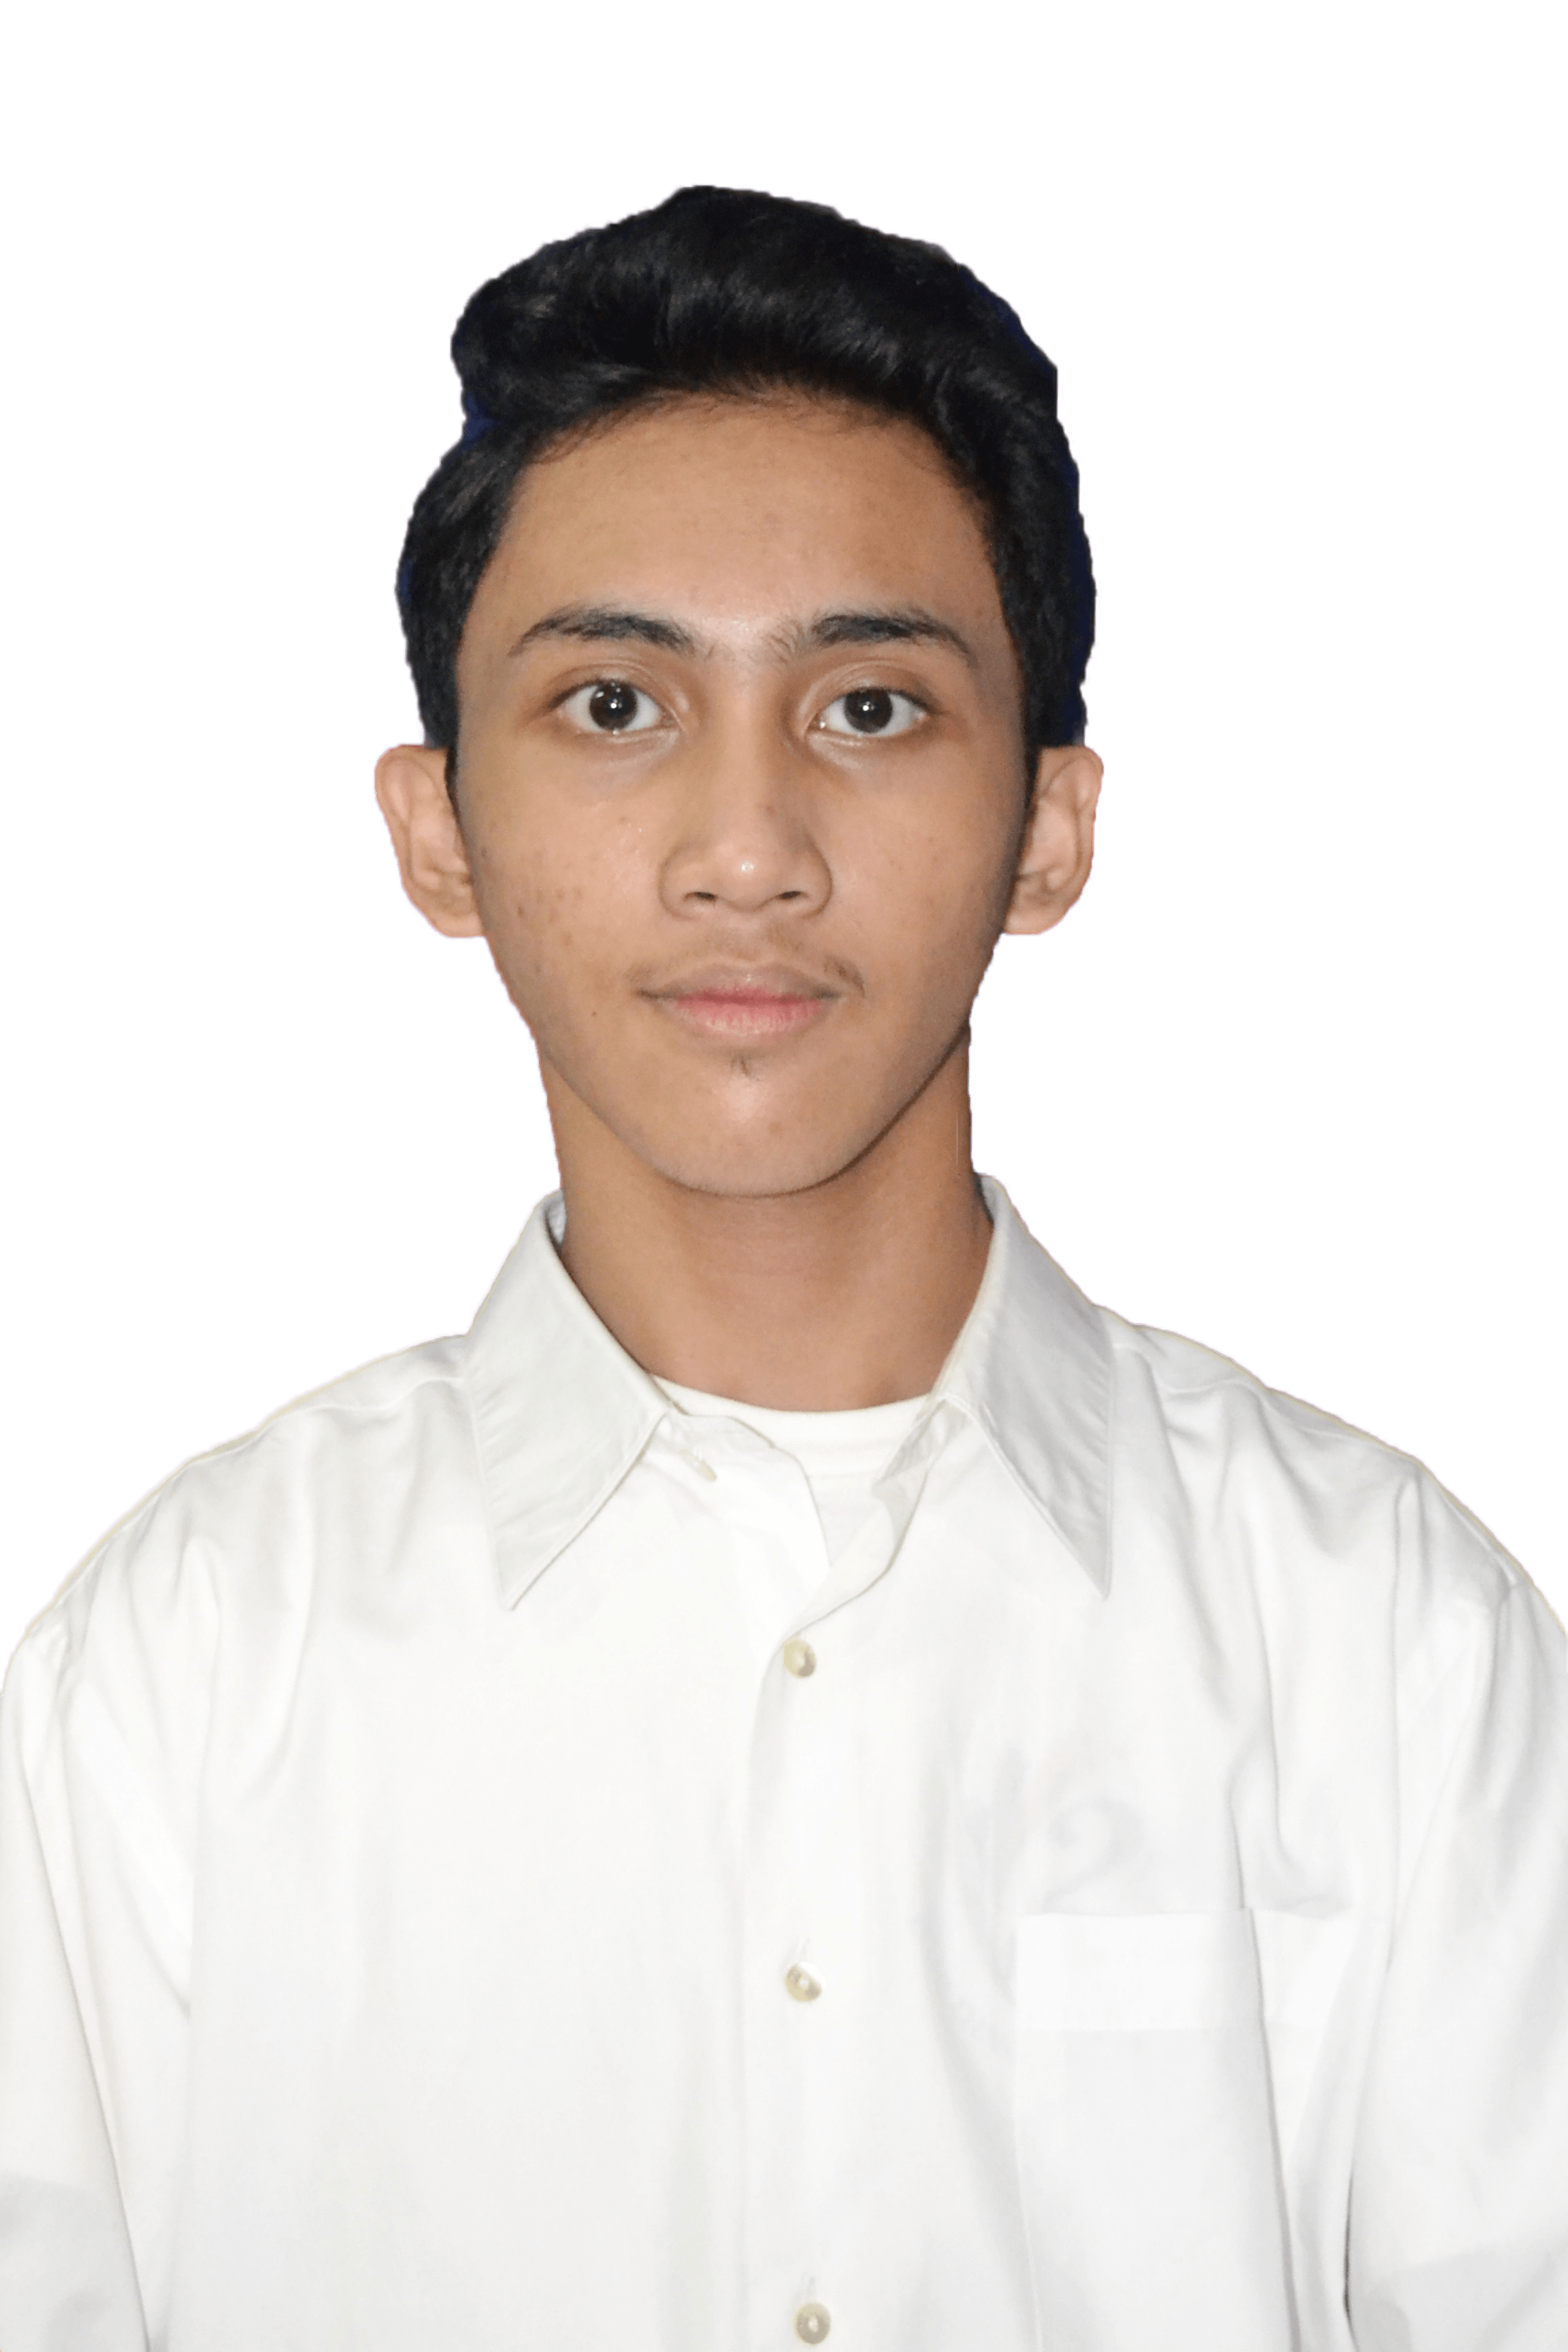
\includegraphics[width=0.3\textwidth]{BiografiPenulis/5024221026_Mahija Ibad Pradipta.png}
	\vspace{-4ex}
\end{wrapfigure}

% Ubah kalimat berikut dengan biografi dari mahasiswa
\name{}, atau yang biasa dikenal sebagai Mahija, lahir di Jakarta Pusat pada 7 Mei 2005. Penulis merupakan anak ketiga dari empat bersaudara yang tinggal dan tumbuh besar di Kota Jakarta. Ketertarikan mendalam penulis di bidang teknologi mengantarkan penulis yang telah menyelesaikan masa sekolah di SMA Negeri 4 Jakarta ke jenjang strata satu di Departemen Teknik Komputer Fakultas Teknologi Elektro dan Informatika Cerdas Institut Teknologi Sepuluh Nopember (ITS) pada tahun 2022.

Penulis merupakan pribadi yang memiliki ketertarikan pada olahraga, ekplorasi alam, maupun menjelajahi topik - topik yang berkaitan dengan bidang teknologi baik software, hardware maupun integrasinya. Ataupun diluar teknologi seperti administrasi, keuangan, dan manajerial. Terbukti dalam masa kuliah, penulis banyak menyelesaikan proyek keperluan tugas mata kuliah yang berkaitan dengan software, hardware, maupun IoT. Selain itu didukung juga dengan rekam jejak organisasi dan kepanitian dari penulis seperti Kepala Divisi Event Multimedia and Game Event (MAGE) X, Kepala Divisi Official Tim Robotika Banyubramanta ITS, Kepala Departemen Kaderisasi HIMATEKKOM ITS 2025/2026. Serta Koordinator Asisten Laboratorium Multimedia dan \emph{Internet Of Things} (IOT). Hingga saat ini penulis masi terus mengembangkan diri baik secara teknis maupun non teknis. 

Pada penelitian tugas akhir ini, penulis memilih mengembangkan drone otonom untuk mendeteksi korban bencana yang berfokus pada integrasi hardware dan software serta penerapan visi komputer. Penulis berharap hasil penelitian ini dapat menjadi kontribusi nyata terhadap pengembangan teknologi pencarian dan penyelamatan di Indonesia. Bagi pembaca yang memiliki kritik, saran, atau pertanyaan mengenai tugas akhir ini dapat menghubungi penulis melalui surel mahijapradipta86@gmail.com.

\cleardoublepage
\end{document}
